\section{Barratt-Puppe sequence}\label{secbarrattpuppe}
%Hood's office hours are from 12 to 1:30 on Mondays in 2-390. Mine are from 4-5 on Tuesday in 2-478. Hood's graded the homework already.
\subsection{Fiber sequences}
Recall, from the previous section, that we have a pullback diagram:
\begin{equation*}
    \xymatrix{
	& F(f,\ast)\ar[r]\ar[d]^p \pb & PY\ar[d]^p\ar[dr]^{\simeq} & \\
	f^{-1}(\ast)\ar[ur]\ar[r] & X\ar[r]_f & Y & \ast\ar[l]
    }
\end{equation*}
Consider a pointed map\footnote{Some people call such a map ``based'', but this makes it sound like we're doing chemistry, so we won't use it.}
$f:X\to Y$ (so that $f(\ast) = \ast$). Then, we will write $Ff$ for the homotopy fiber $F(f,\ast)$.

Since we're exploring the homotopy fiber $Ff$, we can ask the following, seemingly silly, question:
what is the fiber of the canonical map $p:Ff\to X$ (over the basepoint of $X$)?
This is precisely the space of loops in $Y$!
Since $p$ is a fibration (recall that fibrations are closed under pullbacks), the homotopy fiber of $p$ is also the ``strict''
fiber!
Our expanded diagram is now:
\begin{equation*}
\xymatrix{\\
    & \Omega Y=p^{-1}(\ast)\ar[d] & & &\\
    & F(f,\ast)\ar[r]\ar[d]^p & PY\ar[d]^p\ar[dr]^{\simeq} & \\
    f^{-1}(\ast)\ar[ur]\ar[r] & X\ar[r]_f & Y & \ast.\ar[l]
}
\end{equation*}
It's easy to see that the composite $Ff\xar{p} X\xar{f} Y$ sends $(x,\omega)\mapsto f(x)$;
this is a pointed nonconstant map.
(Note that the basepoint we're choosing for $Ff$ is the image of the basepoint in $f^{-1}(\ast)$ under
the canonical map $f^{-1}(\ast)\hookrightarrow Ff$.)

While the composite $fp:Ff \to Y$ is not zero ``on the nose'', it is nullhomotopic, for instance
via the homotopy $h:Ff\times I\to Y$, defined by
$$h(t,(x,\omega)) = \omega(t).$$
\begin{exercise}\label{fiberkernel}
    Let $f:X\to Y$ and $g:W\to X$ be pointed maps.
    Establish a homeomorphism between the space of pointed maps $W \xar{p} Ff$ such that $fp = g$ and the space of pointed
    nullhomotopies of the composite $fg$.
\end{exercise}
This exercise proves that the homotopy fiber is the ``kernel'' in the homotopy category of pointed spaces and pointed
maps between them.

Define $[W,X]_\ast = \pi_0(X^W_\ast)$; this consists of the pointed homotopy classes of maps $W\to X$.
We may view this as a pointed set, whose basepoint is the constant map.
Fixing $W$, this is a contravariant functor in $X$, so there are maps $[W,Ff]_\ast\to [W,X]_\ast\to [W,Y]_\ast$.
This composite is not just nullhomotopic: it is ``exact''!
Since we are working with pointed sets, we need to describe what exactness means in this context:
the preimage of the basepoint in $[W,Y]_\ast$ is exactly the image of $[W,Ff]_\ast\to [W,X]_\ast$.
(This is exactly a reformulation of Exercise \ref{fiberkernel}.)
We say that $Ff\to X\xrightarrow{f}Y$ is a \emph{fiber sequence}.

\begin{remark}
    Let $f:X\to Y$ be a map of spaces, and suppose we have a homotopy commutative diagram:
    \begin{equation*}
	\xymatrix{
	    \Omega Y\ar[d]_{\Omega g}\ar[r] & Ff\ar@{-->}[d]\ar[r] & X\ar[d]_{h}\ar[r]^f & Y\ar[d]^g\\
	    \Omega Y^\prime\ar[r] & Ff^\prime\ar[r] & X^\prime\ar[r]_{f^\prime} & Y.
	    }
    \end{equation*}
    Then the dotted map exists, but it {depends on the homotopy} $f^\prime h\simeq gf$. 
\end{remark}

\subsection{Iterating fiber sequences}
Let $f:X\to Y$ be a pointed map, as before.
As observed above, we have a composite map $Ff\xrightarrow{p} X\xrightarrow{f} Y$, and
the strict fiber (homotopy equivalent to the homotopy fiber) of $p$ is $\Omega Y$.
This begets a map $i(f):\Omega Y\to Ff$; iterating the procedure of taking fibers gives:
\begin{equation*}
    \xymatrix{
	\cdots\ar[r] & Fp_3 \ar[r]^{p_4} & Fp_2\ar[r]^{p_3} & Fp_1\ar[r]^{p_2} & Ff\ar[r]^{p_1} & X\ar[r]^{f} & Y\\
	& \Omega Fp_0\ar[u]|{\simeq}\ar[ur]|{i(p_2)}\ar@{-->}[r] & \Omega X\ar@{-->}[r]\ar[u]|{\simeq}\ar[ur]|{i(p_1)} & \Omega Y\ar[u]|\simeq \ar[ur]|{i(f)} & &
    }
\end{equation*}
All the $p_i$ in the above diagram are fibrations.
Each of the dotted maps in the above diagram can be filled in up to homotopy.
The most obvious guess for what these dotted maps are is simply $\Omega X\xrightarrow{\Omega f}\Omega Y$.
But \emph{that is the wrong map}!

The right map turns out to be $\Omega X\xrightarrow{\overline{\Omega f}}\Omega Y$:
\begin{lemma}
    The following diagram commutes to homotopy:
    \begin{equation*}
	\xymatrix{
	    & Fp\\
	    \Omega X\ar[r]_{\overline{\Omega f}}\ar[ur]^{i(p)} & \Omega Y;\ar[u]
	    }
    \end{equation*}
    here, $\overline{\Omega f}$ is the diagonal in the following diagram:
    \begin{equation*}
	\xymatrix{
	    \Omega X\ar[r]^{-}\ar[dr]|{\Omega f} \ar[d]_{\Omega f} & \Omega X\ar[d]^{\Omega f}\\
	    \Omega Y\ar[r]_{-} & \Omega Y,
	    }
    \end{equation*}
    where the map $-:\Omega X\to \Omega X$ sends $\omega\mapsto\overline{\omega}$.
\end{lemma}
\begin{proof}
    \todo{typeset the following image for the proof... it's going to be impossible to write this up in symbols.}
\begin{figure}[H]
\centering
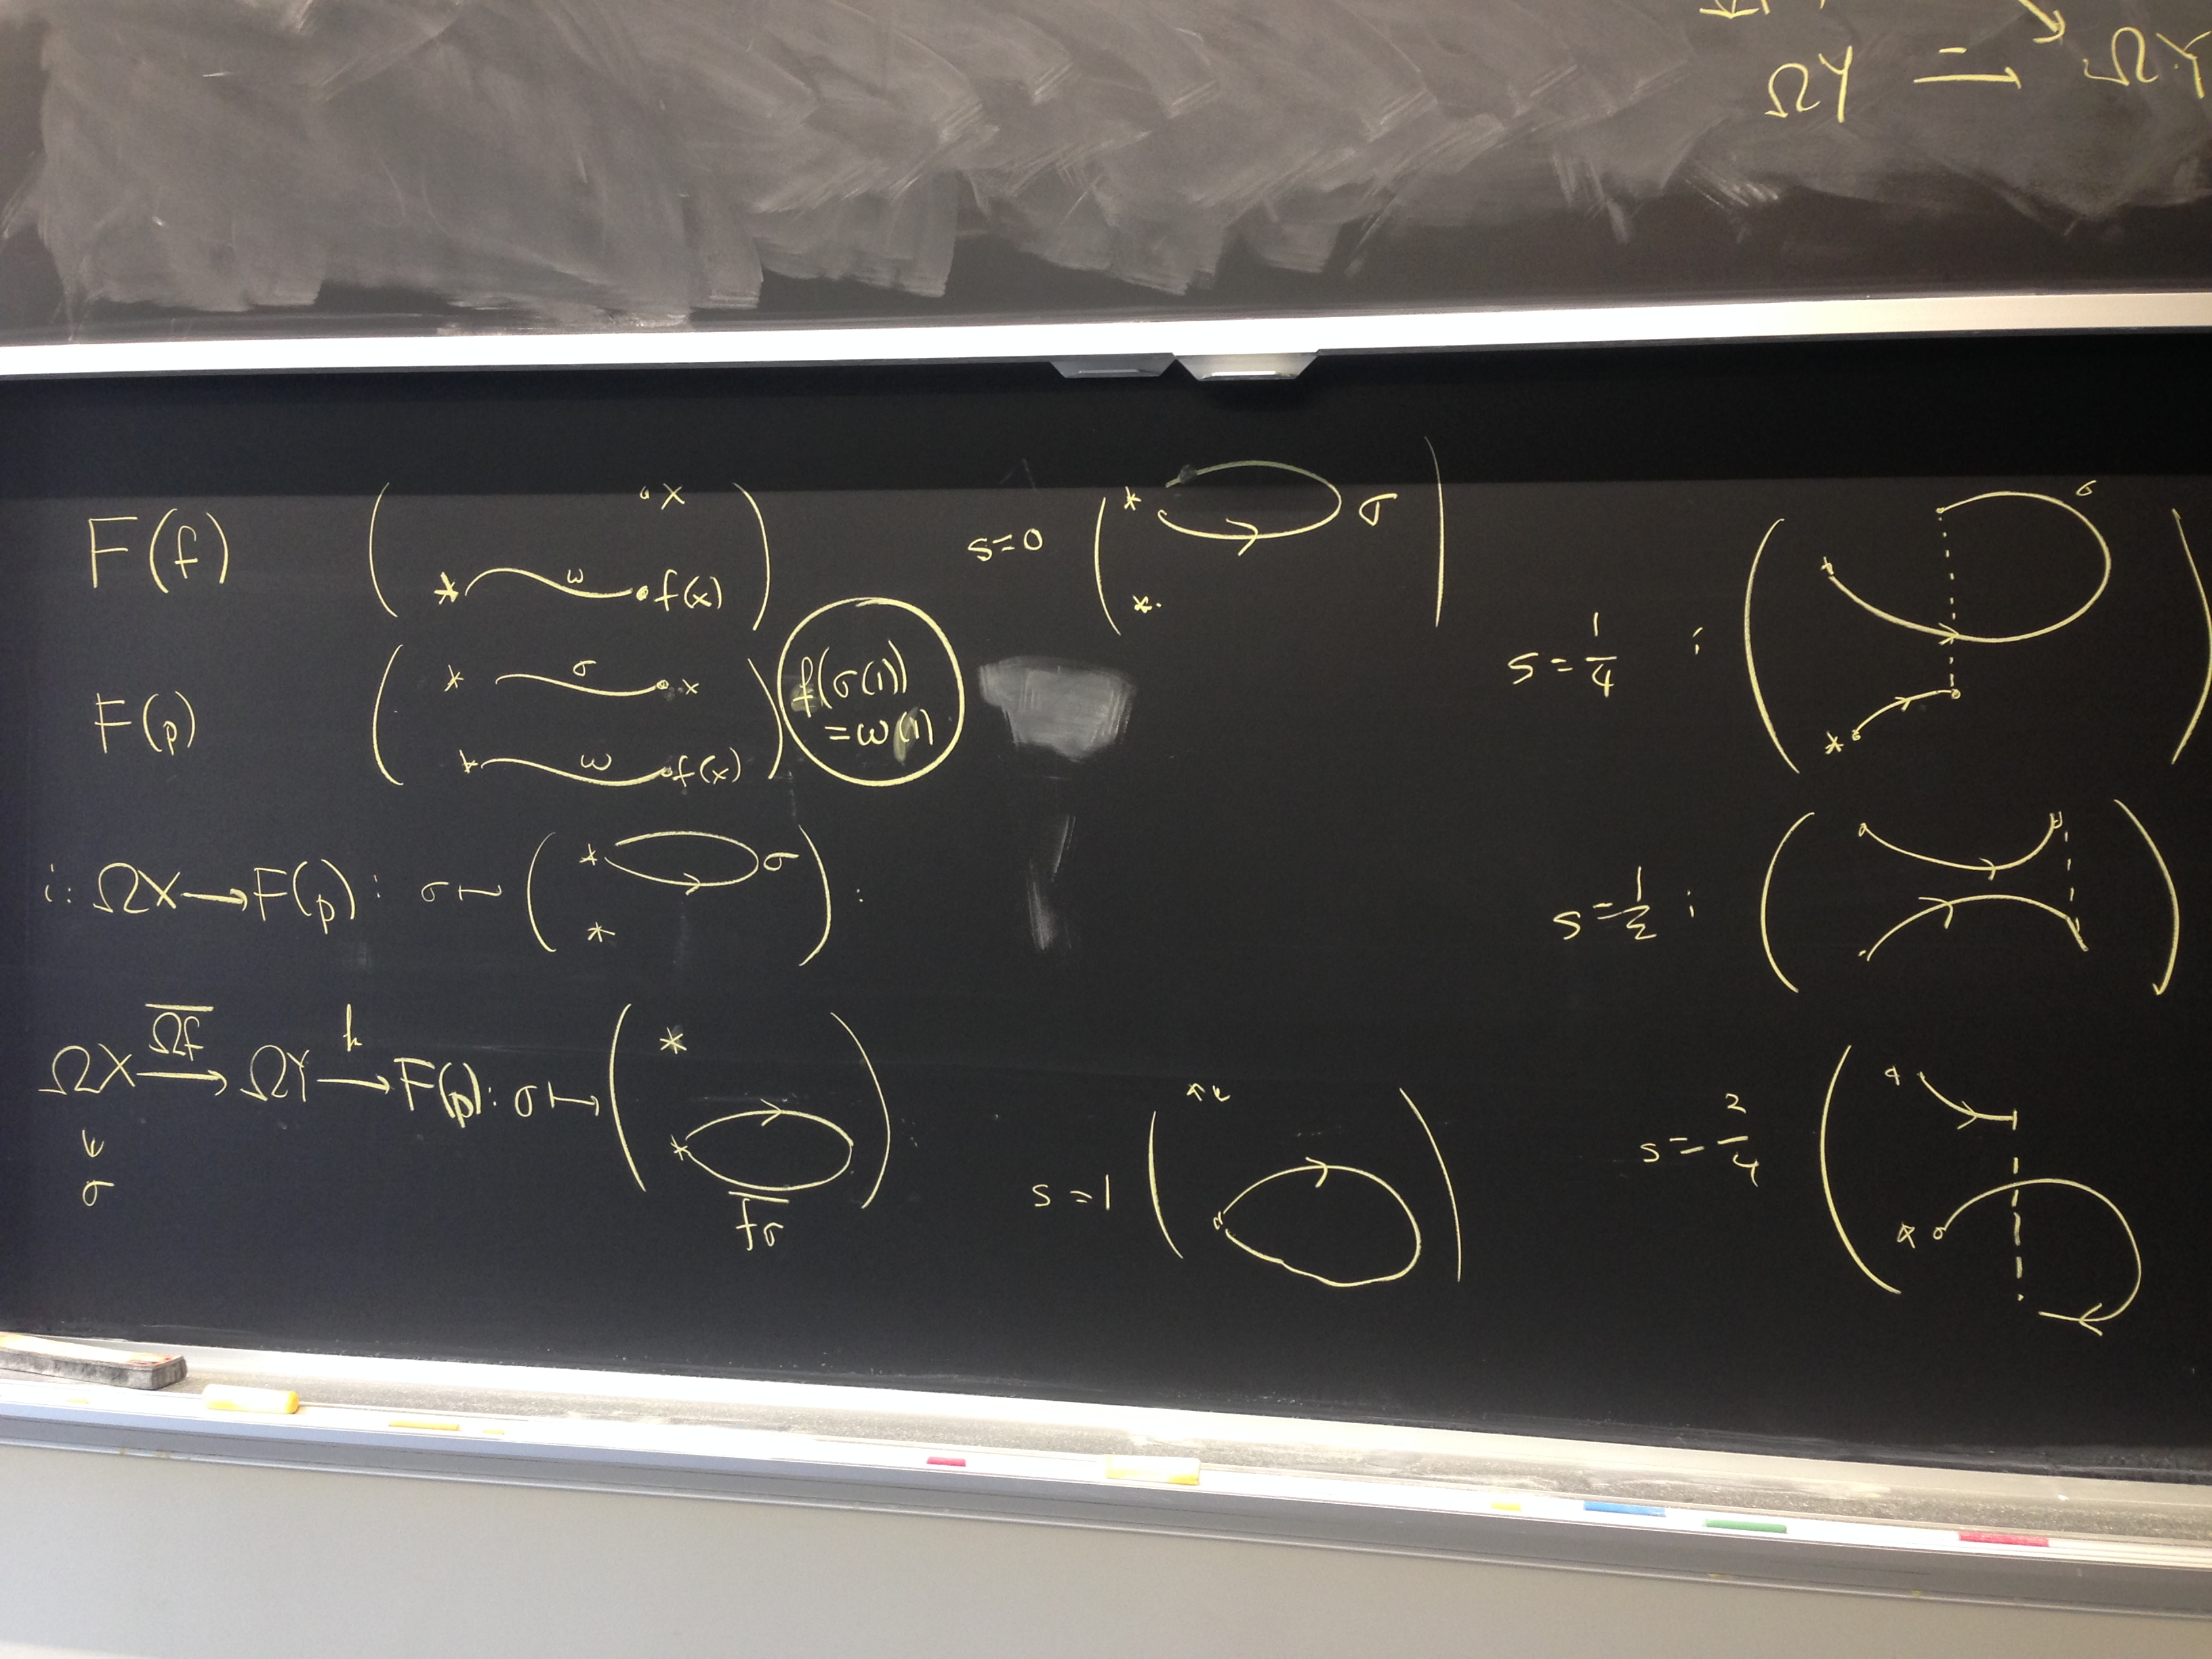
\includegraphics[width=\textwidth]{barratt-puppe}
\caption{A proof of this lemma.}
\end{figure}
\end{proof}
%\begin{lemma}
%    The following diagram commutes:
%    \begin{equation*}
%	\xymatrix{
%	    & F(\overline{\Omega p_0})\ar@{=}[dd]\ar[dr] & \\
%	    \Omega^2 Y\ar[ur]^{i(\Omega p_0)}\ar[dr]_{\overline{\Omega i(p_0)}} & & \Omega X\\
%	    & \Omega Fp_0\ar[ur]_{\overline{\Omega p_1}} & 
%	    }
%    \end{equation*}
%\end{lemma}
%What is the map $F\overline{\Omega p_0}\to \Omega X$?? We spent some time figuring this out.
%But you can now apply $[W,-]_\ast$ to the following diagram to get a long exact sequence:
By the above lemma, we can extend our diagram to:
\begin{equation*}
    \xymatrix{
	\cdots\ar[r] & Fp_4\ar[r] & Fp_3 \ar[r] & Fp_2\ar[r] & Fp_1\ar[r]^{p_2} & Ff\ar[r]^{p_1} & X\ar[r]^{f} & Y\\
    \cdots\ar[r] & \Omega Fp_1\ar[r]|{\overline{\Omega p_2}}\ar[u]_{\simeq} & \Omega Ff\ar[u]_{\simeq}\ar[ur]|{i(p_2)}\ar[r]|{\overline{\Omega p}} & \Omega X\ar[r]|{\overline{\Omega f}}\ar[u]_{\simeq}\ar[ur]|{i(p_1)} & \Omega Y\ar[u]_\simeq \ar[ur]|{i(f)} & &\\
	\Omega^2 X\ar[u]_{\simeq}\ar[r]_{\Omega^2 f} & \Omega^2 Y\ar[u]_{\simeq}\ar[ur]_{\overline{\Omega i(p_0)}} & & &
    }
\end{equation*}
We have a special name for the sequence of spaces sneaking along the bottom of this diagram:
$$\cdots\to \Omega^2 X \to \Omega^2 Y \to \Omega Ff \to \Omega X \to \Omega Y \to Ff \to X \xar{f} Y;$$
this is called the \emph{Barratt-Puppe sequence}.
Applying $[W,-]_\ast$ to the Barratt-Puppe sequence of a map $f:X\to Y$ gives a long exact sequence.

The most important case of this long exact sequence comes from setting $W = S^0=\{\pm 1\}$;
in this case, we get terms like $\pi_0(\Omega^n X)$.
We can identify $\pi_0(\Omega^n X)$ with $[S^n,X]_\ast$: to see this for $n=2$,
recall that $\Omega^2 X = (\Omega X)^{S^1}$; because $(S^1)^{\wedge n} = S^n$ (see below for a proof of this fact), 
we find that
\begin{equation}\label{bpsequence}
(\Omega X)^{S^1} \simeq (X^{S^1}_\ast)^{S^1}_\ast = X_\ast^{S^1\wedge S^1} = X_\ast^{S^2},
\end{equation}
as desired.

The space $\Omega X$ is a group in the homotopy category; this implies that
$\pi_0 \Omega X = \pi_1 X$ is a group!
For $n>1$, we know that
$$\pi_n(X) = [(D^n,S^{n-1}),(X,\ast)] = [(I^n,\partial I^n),(X,\ast)].$$
\begin{exercise}
    Prove that $\pi_n(X)$ is an abelian group for $n>2$.
\end{exercise}
%Suppose $n=2$, for simplicity.
%How do I take the product of $\alpha,\beta\in \pi_2(X)$?
%Thinking of $\pi_2(X)$ as $[(I^2,\partial I^2),(X,\ast)]$ tells us that . You can play this game; up to homotopy, you can shrink $\alpha$ and $\beta$ to make them as small I want, and then reverse their position and expand them again\footnote{This probably makes no sense without a picture}\todo{Add a picture}. Thus $\pi_2(X)$ is an abelian group.
Applying $\pi_0$ to the Barratt-Puppe sequence (see Equation \ref{bpsequence}) therefore gives a long exact sequence
(of groups when the homotopy groups are in degrees greater than $0$, and of pointed sets in degree $0$):
$$\cdots\to \pi_2 X\to \pi_2 Y\to \pi_1 Ff\to \pi_1 X\to\pi_1 Y\to\pi_0 Ff\to\pi_0 X\to \pi_0 X.$$
